\begin{frame}{A path with many options}
 \begin{itemize}
  \item There are many different options to choose
  \item I explain my choices but dicuss other options
  \item Goal: Be clear so other researchers can adapt my methodology to their problems
 \end{itemize}

\end{frame}

\begin{frame}{MI primer}
\begin{itemize}
 \item MI forms the base of this thesis
 \item There are lots of different ways to impute
 \item As long as we can impute valid imputations, we can analyze them
 \item Poor imputation leads to poor results (bias, variability, loss in power)
\end{itemize}
\end{frame}

\begin{frame}{MI Notation}
 
 \begin{itemize}
\item $Y$ is our whole dataset. It will have $i$ rows and $j$ columns. Some of the covariates in the dataset will be completely observed, and others will have missingness.
\item $Y_j$ is a specific column of Y. $Y_j$ is composed as $Y_j=(Y_{j,obs},Y_{j,mis})$, where
	\begin{itemize}
	\item $Y_{j,obs}$ is the data we have observed for covariate j
	\item $Y_{j,mis}$ is the missing data covariate j
\end{itemize} 
\item $Y_{obs}$ is all of the data that we have observed
\item $Y_{mis}$ is all the data that we have not observed
\item R is a binary matrix the same size as $Y$ where a 1 indicates we observed the data, and 0 means it is missing
\item $\psi$ is a vector of parameters for the missing data model. 
\item The missing data model is given as $p(R|Y_{obs},Y_{mis},\psi)$
\item $\theta$ is a vector of the parameters for the full model of $Y$
\end{itemize}
\end{frame}

\begin{frame}{MI Concepts}
\begin{itemize}
 \item Ignorability
$$p(Y_{mis}|Y_{obs},R)= p(Y_{mis}|Y_{obs})$$
That is, we may ``ignore'' the R. The probability of the data being missing does not depend on how the data is missing. 
Equivalently, we may write this as
$$p(Y_{mis}|Y_{obs},R=1)= p(Y_{mis}|Y_{obs},R=0)$$
\item Non ignorability: $$p(Y_{mis}|Y_{obs},R=1)\neq p(Y_{mis}|Y_{obs},R=0)$$
So we must take into account the missing data structure for imputation.


\end{itemize}

\note{Being ignorable makes it justified to model our missing data from our observed data, without needing to worry about how it was missing.
The opposite of ignorable data is called non-ignorable data, in this case.
We often times see ignorable missing data in practice,
although one should certainly check the sensibility of ignorability, as some instances will certainly be non-ignorable, 
for example censored data, or when we know that the missing data is systematically different than the observed. 
If we have strongly nonignorable data, we should either try one of two things.

The first is to expand the data (collect something else similar to the covariate with missingness) so that it becomes ignorable and 

the second is to formulate two imputation models, one for the observed and one for the missing.

}

\end{frame}

\begin{frame}{Missing data Mechanisms}
Now, we may discuss the three main types of missing data mechanisms. 
\begin{itemize}

\item MCAR: Missing completely at random:  $$P(R=0|Y_{obs},Y_{mis},\psi)=P(R=0|\psi)$$
\begin{itemize}
\item The missingness in the data is not at all related to any of the data that we do or don't have
\end{itemize}
\item MAR: Missing at random: $$p(R=0|Y_{obs},Y_{mis},\psi)= p(R=0|Y_{obs},\psi)$$
\begin{itemize}
 \item The missingness we have is related to something in the data 
\end{itemize}
\item MNAR: Missing not at random: $$p(R=0|Y_{obs},Y_{mis},\psi)$$ does not simplify
\begin{itemize}
 \item  and the missingness depends on data that we have as well as have not collected
\end{itemize}


\end{itemize}
\note{
 If a lab technician slips and drops 5 vials of blood, the missingness caused by this would be MCAR
 If we collect the gender of the subject and we know that males tend to not give blood, we can attribute the missingness to the gender. In general, MAR models are ignorable.
 For example if a full moon causes the blood testing machine to break more often, but we don't have the moon phase as a variable.
}
 
\end{frame}

\begin{frame}{Joint Modelling}
 \begin{itemize}
  \item Assume ignorable MAR  missing data mechanism
  \item Missing data imputed by sampling from a user specified distribution
  \item A lot of theory developed for Normal, not much else
  \begin{itemize}
   \item Normal imputation has been shown to perform well, even under non normality \cite{Demirtas2008}
  \end{itemize}
\item Idea: pull imputations by missing data row pattern
 \end{itemize}

\end{frame}

\begin{frame}{JM pseudocode}
 \begin{figure}[h!]
  \centering
    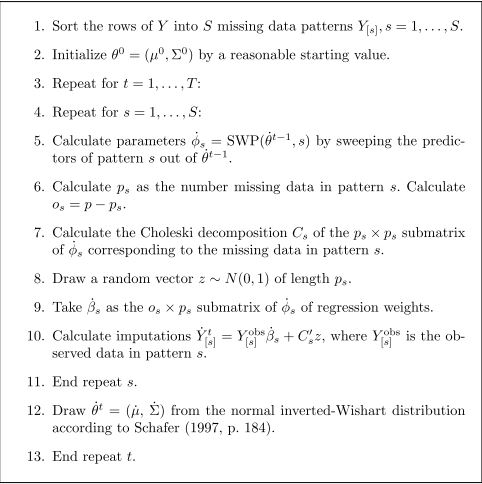
\includegraphics[width=0.6\textwidth]{jm_algo}
 % \caption{Normal JM imputation pseudocode}
\label{fig:jmexample}
\end{figure}
%do I want to include the amelia algo?
\end{frame}

\begin{frame}{JM Pros and Cons}
Pros
 \begin{itemize}
  \item Fast
  \item Easy to derive posteriors with common distributions
 \end{itemize}

 Cons
 \begin{itemize}
  \item Inflexible
  \item Limited to known distributions
  \item How to deal with mixed categorical and continous missing data
 \end{itemize}

\end{frame}

\begin{frame}{Full Conditional Specification}
 \begin{itemize}
  \item Assume MAR missing data mechanism %althouth MNAR with more 
  \item Missing data is imputed iteratively on a variable by variable basis
  \item Requires no distributional assumptions
  \item Idea: Specify k one dimensional models to impute on the missing data columns
 \end{itemize}

\end{frame}

\begin{frame}{FCS Algorithm}
  \begin{figure}[h!]
  \centering
    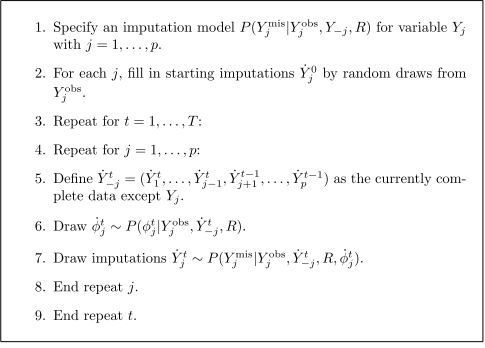
\includegraphics[width=0.6\textwidth]{fcs_algo}
 % \caption{Normal JM imputation pseudocode}
\label{fig:fcsexample}
\end{figure}
 \note{ Observe how the previous imputation Y_j^(t-1) only enters the current imputation
 through its relation with other variables, and not directly. This makes convergence very fast
}
\end{frame}

\begin{frame}{FCS Pros and Cons}
Pros
 \begin{itemize}
  \item Flexible
  \item Easy to specify models
  \item Handles mixed continous categorical
 \end{itemize}

 Cons
 \begin{itemize}
  \item No guarantee that full conditionals are compatible
  \item Slow
  \item Gets much harder as sample size increases to specify models
 \end{itemize}

\end{frame}